\begin{figure}[htbp]
	\centering
	\begin{minipage}[t]{0.48\textwidth}
		\centering
		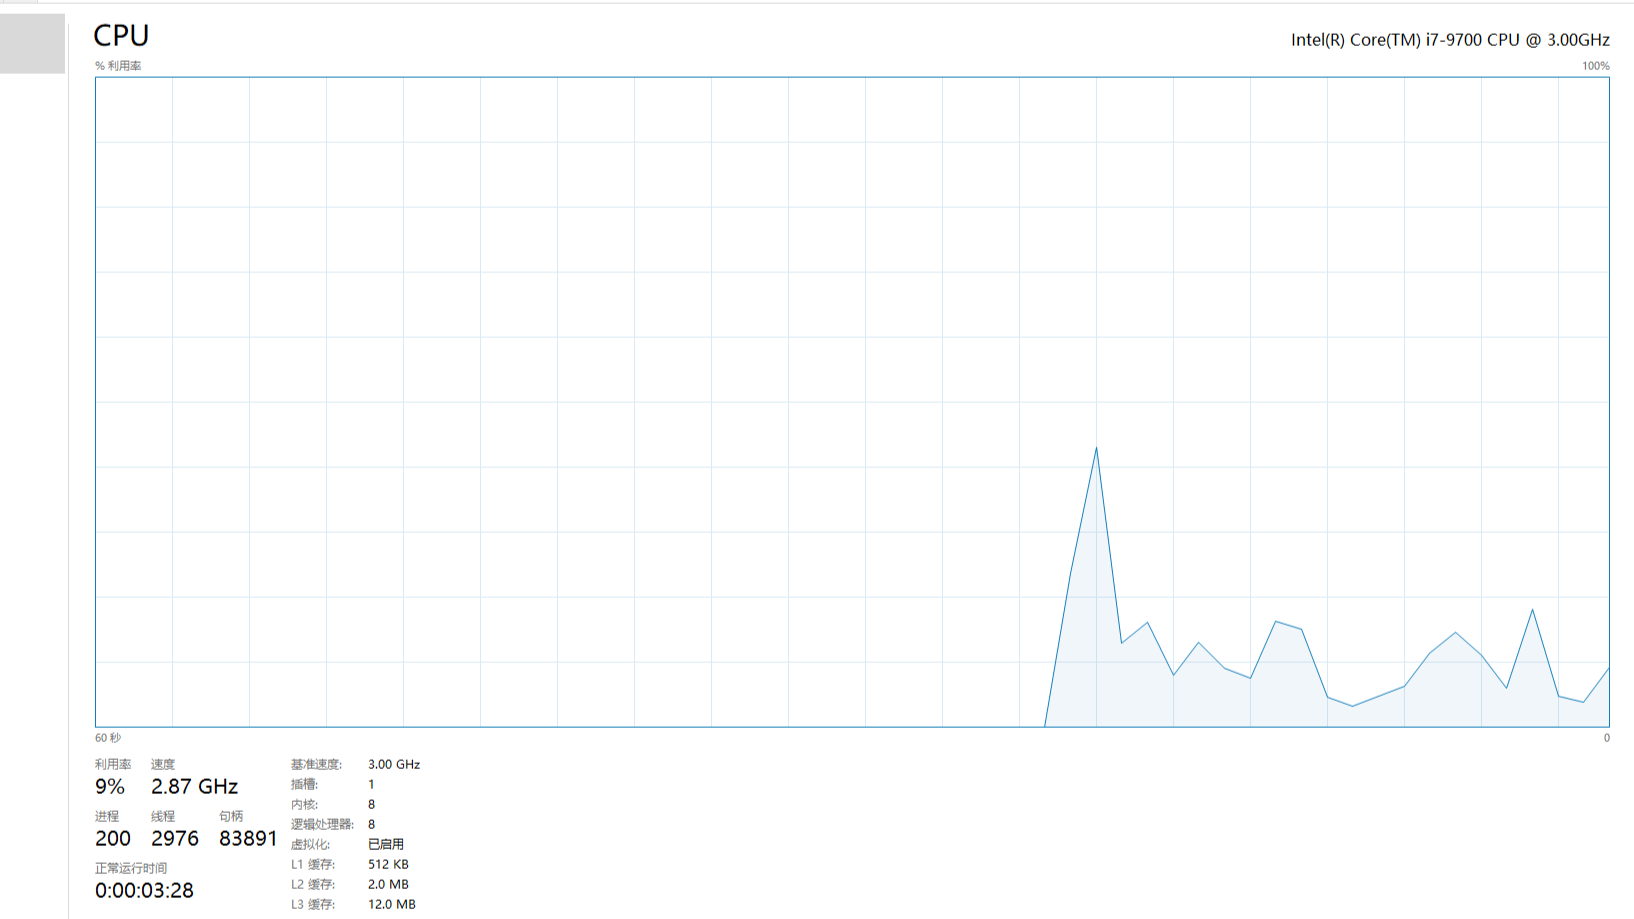
\includegraphics[width=1\textwidth]{figures/device_para/cpu.png}
		\caption{CPU参数}
		\label{fig:cpupara}
	\end{minipage}
	\begin{minipage}[t]{0.48\textwidth}
		\centering
		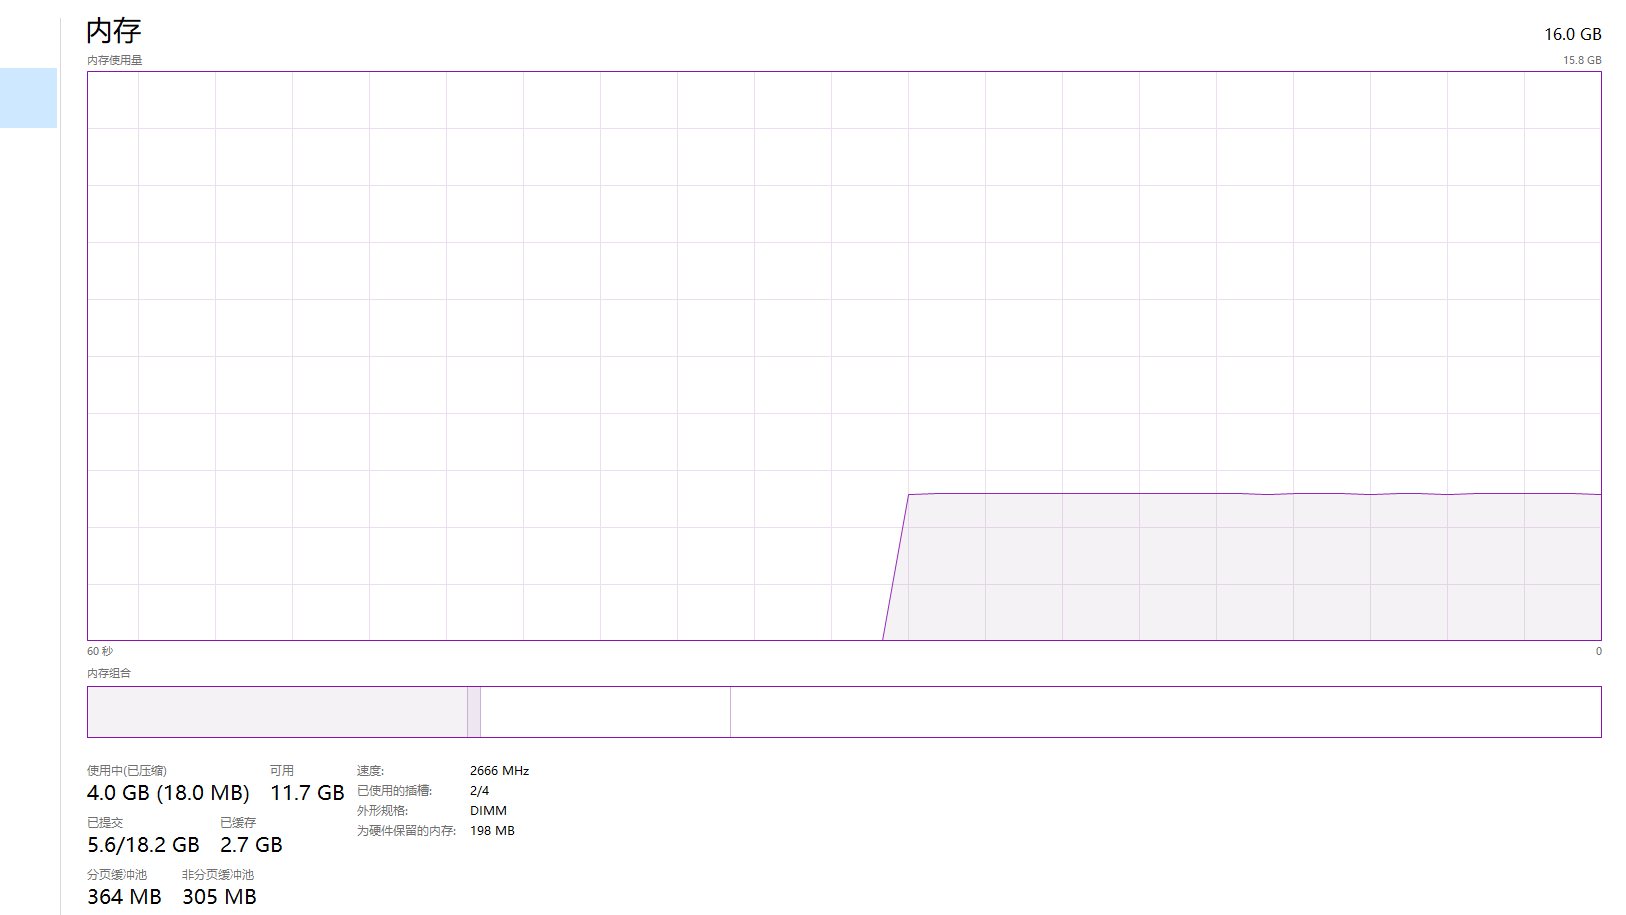
\includegraphics[width=1\textwidth]{figures/device_para/ram.png}
		\caption{RAM参数}
		\label{fig:rampara}
	\end{minipage}

	\centering
	\begin{minipage}[t]{0.48\textwidth}
		\centering
		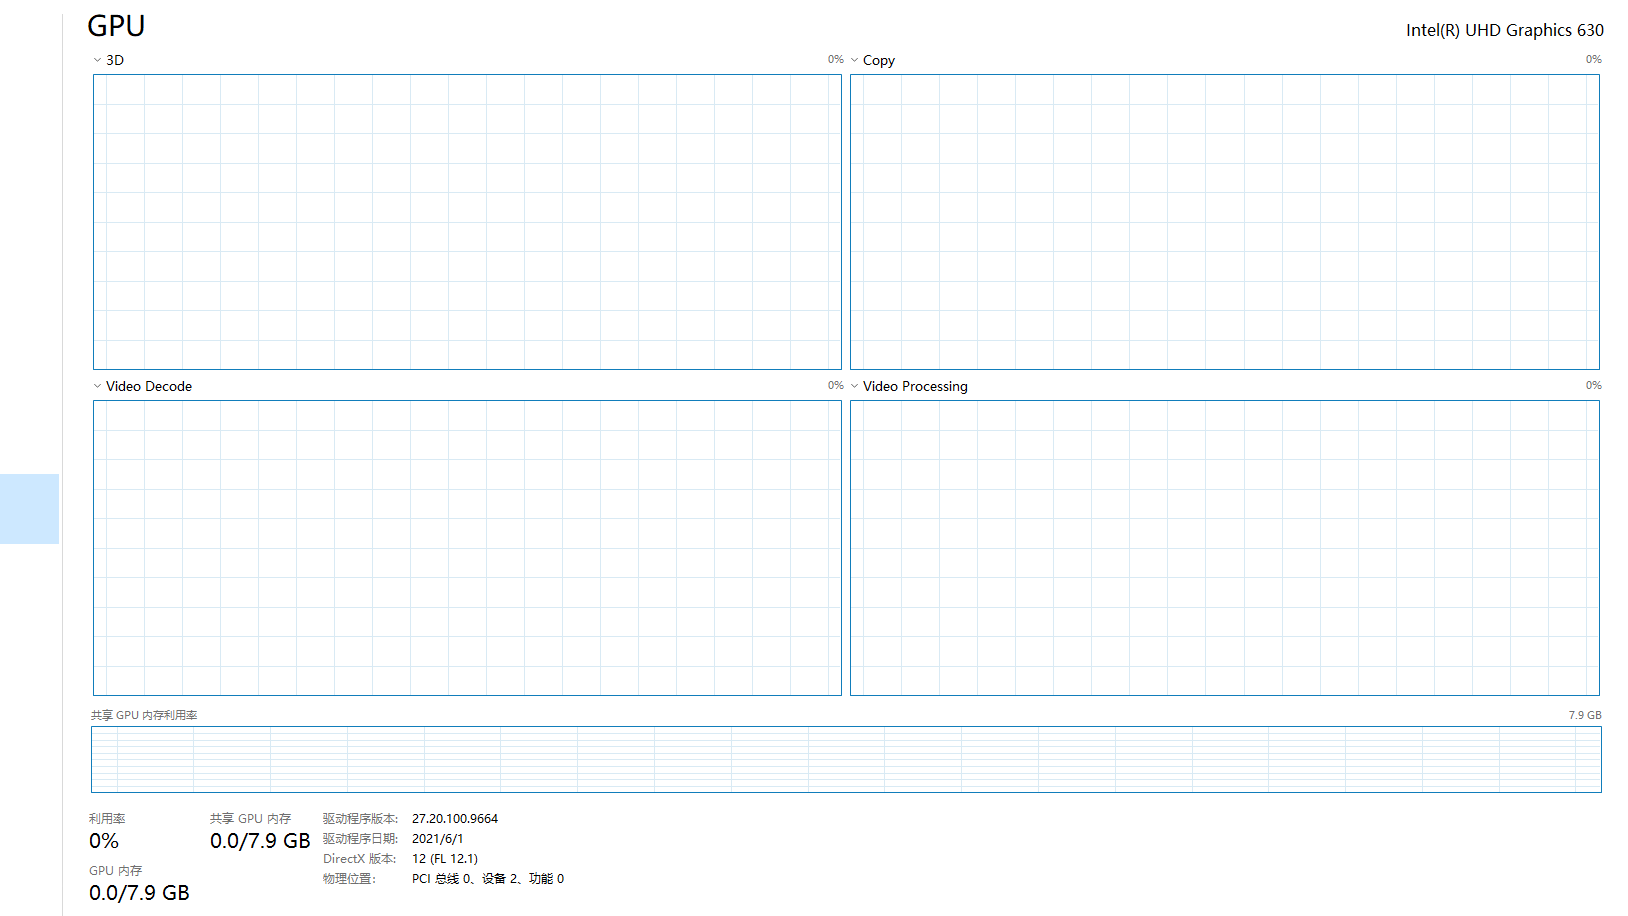
\includegraphics[width=1\textwidth]{figures/device_para/igp.png}
		\caption{IGP参数}
		\label{fig:igppara}
	\end{minipage}
	\begin{minipage}[t]{0.48\textwidth}
		\centering
		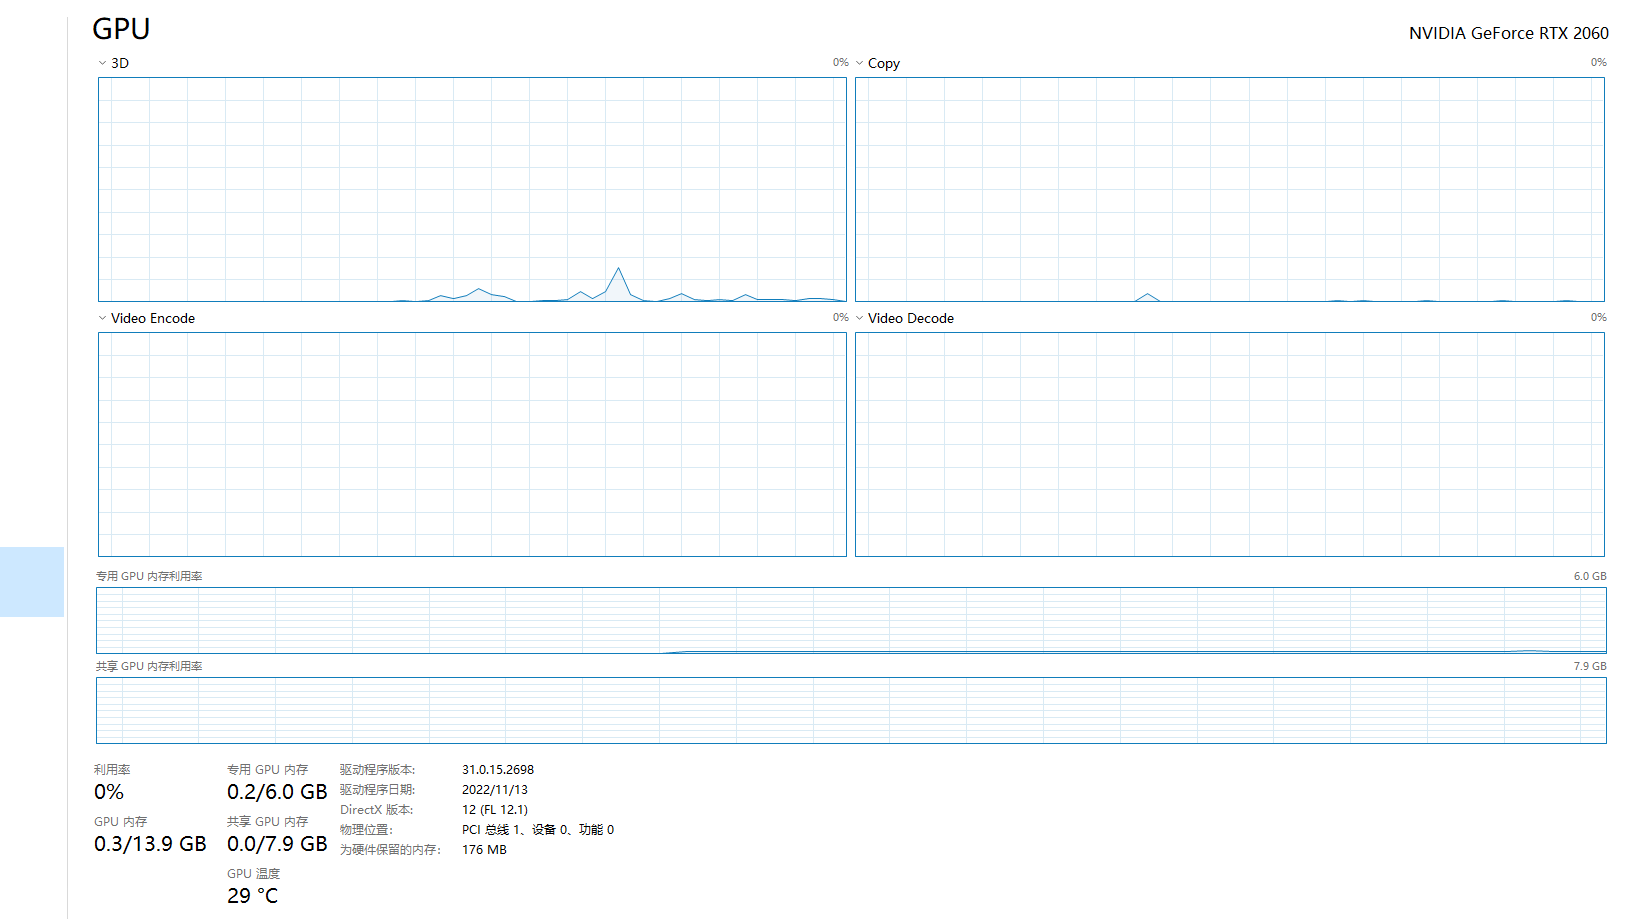
\includegraphics[width=1\textwidth]{figures/device_para/gpu.png}
		\caption{GPU参数}
		\label{fig:gpupara}
	\end{minipage}
\end{figure}

\begin{enumerate}
	\item{硬件环境}
	\par Intel Core i7-9700 CPU,16GB 内存(RAM),Intel(R) UHD Graphics 630集成图形处理器(IGP)和NVIDIA GeForce RTX 2060 GPU。所有计算均在此硬件环境上完成。
	具体信息见图\ref{fig:cpupara} $\sim$ 图\ref{fig:gpupara}。

	\item{操作系统}
	\par Windows 10 专业版 22H2 和 Ubuntu 20.04 LTS为主要的开发和运行环境,因其对开源软件和库支持良好。

	\item{开发语言}
	\par C++14和Python3.9。Python用于实现RGB图像语义分割,C++用于实现系统其他的所有功能。

	\item{开发工具}
	\par 使用Visual Studio Code 1.78和NVIDIA Nsight Compute 2022作为代码编辑器,CUDA 11.8进行GPU并行计算的开发,使用Git进行版本控制。

	\item{编译器}
	\par 使用GCC 11.3.0编译Ubuntu系统的C++代码,NVCC 11.7编译CUDA代码,以及MSVC 14.3编译Windows系统的C++代码。

	\item{依赖库}
	\par OpenCV 4.6用于图像处理,Open3D 0.16用于点云后处理,OpenGL 3.3和GLFW 3.3.8用于图形渲染和窗口管理,以及Intel Realsense SDK 2.0用于操作Intel Realsense相机。
\end{enumerate}